\chapter{Projektowanie i implementacja}
\label{cha:implementacja}

Nakreślony problem -- rozproszonego systemu, który dzięki propagacji danych między użytkownikami obniży obciążenie serwerów sieci Web -- stawia wiele wyzwań projektowych i architektonicznych.

\section{Wymagania funkcjonalne}
\label{sec:funkcjonalnosc}

System dHTTP, z punktu widzenia użytkownika, ma spełniać jedną funkcjonalność: utrzymać lub poprawić płynność dostępu do interesujących go witryn internetowych, nie wpływając na ich treść i nie naruszając prywatności.

Projekt udostępnia interfejs zapewniający dostęp do statystyk, a także preferencji użytkownika. Udostępnione preferencje dotyczą: stopnia działania aplikacji w tle, trybów propagacji i przechowywania danych.
% To może powinno być gdzieś indziej
\begin{figure}[h]
	\centering
    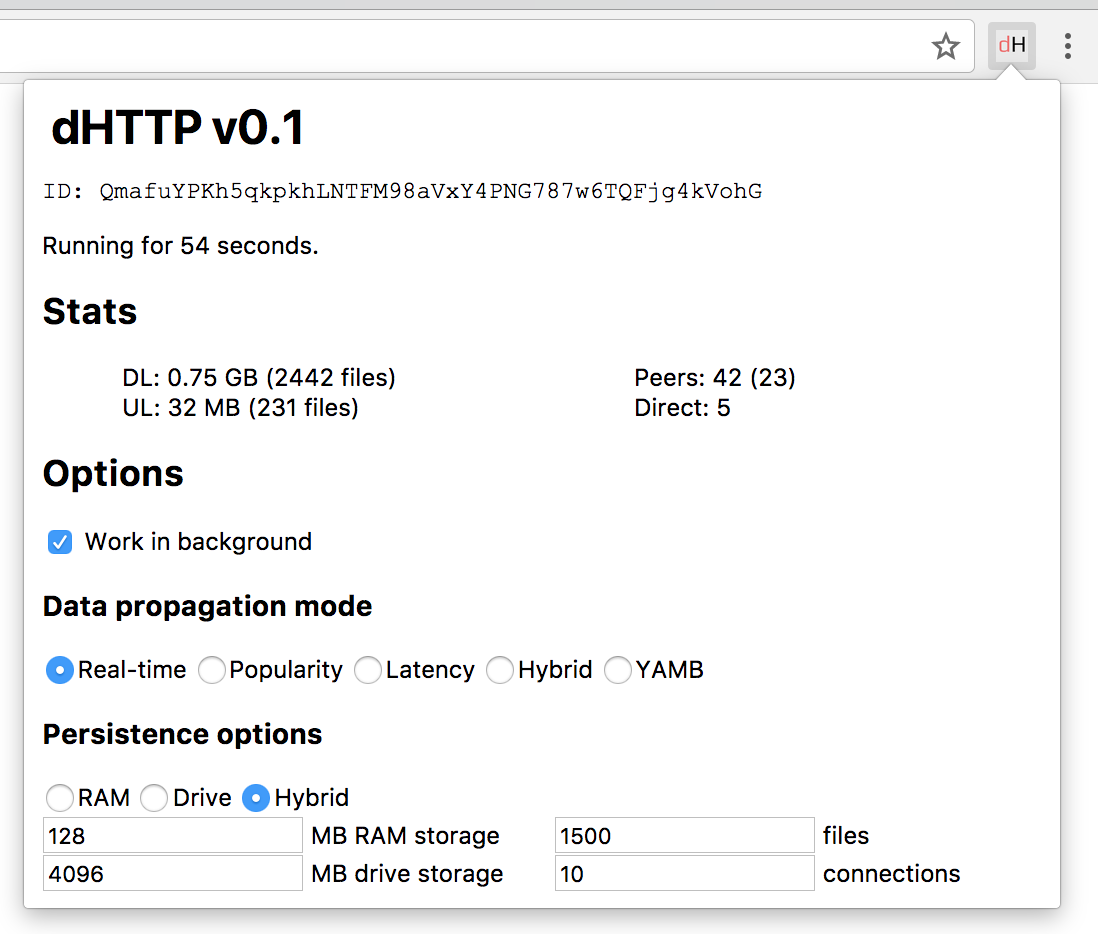
\includegraphics[scale=0.5]{dhttp-initial-interface.png}
	
	\caption{\label{fig:initialInterface} Wstępna implementacja interfejsu operacji dla systemu dHTTP: pop-up dostarczany przez wtyczkę do przeglądarki Google Chrome pozwala na obserwację statystyk i zmianę preferencji.}
\end{figure}

% TODO - gdzieś w pracy podkreśl, jak bardzo istotna jest prosta i automatyczna klastryzacja
Wymogiem dla projektu, koniecznym z racji potrzeby prostej automatyzacji rozrostu sieci, jest tryb niezależny aplikacji -- {\em headless mode} -- pozwalający na wystartowanie niezależnego węzła jednym poleceniem. Niezbędnym jest, aby węzeł tego typu udostępniał statystyki użycia i wstępną konfigurację przy użyciu poleceń interfejsu konsolowego, pozwalając jednak na funkcjonalne uruchomienie z domyślną konfiguracją.


\section{Definicje, architektura i technologie}
\label{sec:zalozeniaProjektu}

\subsection{Słownik pojęć}

W celu uniknięcia niejednoznaczności w dalszym toku pracy, zdefiniowane zostaną następujące pojęcia:

\begin{itemize}
    \item \textbf{węzeł} -- pojedynczy, autonomiczny element systemu, który wykorzystuje komunikację sieciową w celu rozgłaszania i pobierania danych;
    \item \textbf{klient} -- węzeł, który pobiera dane w celach użytkowych, zaimplementowany w wersji dedykowanej użytkownikowi końcowemu;
    \item \textbf{klaster} -- zbiór węzłów, który posiada informacje i ścieżki komunikacyjne pozwalające efektywnie na wymianę informacji pomiędzy każdym z nich;
    \item \textbf{metadane klastra} -- ustrukturyzowane informacje wymieniane pomiędzy węzłami w celu ustalenia stanu i optymalizacji działania klastra;
    \item \textbf{metadane pliku} -- ustrukturyzowane informacje wymieniane między węzłami w celu propagacji i umożliwienia wymiany faktycznych danych plikowych;
  \end{itemize}
      % TODO - dodać nowe, jeśli się pojawią/przyjdą do głowy

\subsection{Koncept architektury}

Z punktu widzenia klastra, koncepty węzła i klienta są jednoznaczne i równorzędne -- wszystkie wyposażone są we wspólne mechanizmy komunikacji, i protokół wymiany danych między nimi działa na niezmienionej zasadzie. Wspólnie budować będą rozproszoną tablicę haszującą (DHT), która pozwoli na dostęp do metadanych klastra, które informować będą o cechach poszczególnych węzłów, oraz metadanych plików, przyspieszając proces ich identyfikacji i zapewniając oraz bezpieczeństwo spójność danych.

W celu zapewnienia płynności działania systemu, metadane klastra powinny zawierać w sobie informacje o {\em reputacji} poszczególnych węzłów. Podczas gdy węzły serwerowe z reguły zostają uruchomione i będą działać, mając szczyty obciążenia czy wymagań zależne głównie od obciążenia całej sieci (lub ewentualnego alternatywnego oprogramowania serwerowego na nich uruchamianego), węzły klienckie podlegać będą prawdopodobnie o wiele większej dynamice, z racji częstych odczytów dużych plików i podejścia użytkownika, które może zakładać częste otwieranie i zamykanie przeglądarki.

Węzły serwerowe i klienci powinny mieć zatem różne wartości bazowe przy ocenie ich sprawności w sieci -- reputacja oprogramowania klienckiego powinna być domyślnie niższa, i szybciej reagować na zmiany jej wartości.

\subsection{Wykorzystane technologie i narzędzia}
\label{sec:techNTools}
% akapit poniżej prawdopodobnie jest o wiele lepszą kanwą dla czegoś w części teoretycznej niż czymś, co powinno być tutaj.

Budowa kompletnego stosu technologicznego dla projektu o takich wymaganiach przez lata pozostawała problemem nietrywialnym. Paradygmaty programowania specjalizowane w podejściu obiektowym wspierały budowę monolitów, a komunikacja klient-serwer często polegała na tworzeniu dużej ilości poleceń, bez skupienia na wydajności takich rozwiązań.

Dużą zmianą w tej kwestii jest rozwój \texttt{libp2p}, stanowiący efekt długotrwałej pracy nad zrozumieniem stosu sieciowego Internetu, zbiór protokołów i wyprowadzonych zeń narzędzi, mechanik i interfejsów, pozwalających na ich podstawie budować własne, kompleksowe rozwiązania (\cite{libp2p-specs}).

\texttt{libp2p} stanowi względnie wysokopoziomową kanwę dla projektu dHTTP. To właśnie na efektach pracy tego projektu opiera się warstwa tworzenia i komunikacji węzłów, budująca klaster dHTTP. Implementacja \texttt{js-libp2p} udostępnia moduły niezbędne w komunikacji sieciowej, łączeniu strumieni różnych protokołów, wykrywaniu nowych węzłów, propagowaniu informacji o istniejących węzłach sieci czy wreszcie budowaniu rozproszonej tablicy haszującej, stanowiącej bazę metadanych klastra i plików.

Nie bez wpływu pozostaje rozwój przeglądarek internetowych. Współczesne browsery udostępniają kompleksowe API, pozwalające rozwijać wtyczki zmieniające zawartość stron internetowych, z uwzględnieniem kwestii wydajności i bezpieczeństwa. Istotne jest również wsparcie dla nowych technik komunikacji takich jak {\em WebSockets}, pozwalającej na wymianę informacji w czasie rzeczywistym, dzięki utrzymywaniu dwustronnie interaktywnej sesji TCP pomiędzy przeglądarką i serwerem.
% TODO cite https://developer.chrome.com/extensions lub bardziej specyficznie.

Za powstanie {\em headless} dHTTP w znacznej części odpowiada Node.js -- środowisko uruchomieniowe pozwalające na uruchamianie kodu JavaScript po stronie serwerowej.  Narzędzia, takie jak \texttt{npm} i Browserify, pozwalają z kolei na wykorzystywanie serwerowego kodu JavaScriptu w kodzie klienckim. Dzięki możliwości rozwoju obu aplikacji przy użyciu tego samego języka programowania i powyższym rozwiązaniom, znaczna część  kodu aplikacji może być współdzielona.

% Języki programowania nie były zaadaptowane do prostej komunikacji sieciowej, a przeglądarki nie wspierały krytycznych narzędzi i protokołów pozwalających na komunikację w czasie rzeczywistym, pozostawiając problemy natury wydajnościowej uniemożliwiające użyteczną implementację tego typu rozwiązań.


% istnieje ryzyko, że ten akapit będzie musiał znaleźć swoje miejsce trochę gdzieś indziej
\subsection{Problemy warstwy sieciowej}
\label{sec:networkIssues}

Choć przeglądarki coraz chętniej


\subsection{Decentralizacja czy rozproszenie?}
\label{sec:decentralizacjaCzyRozproszenie}

\subsection{Bezpieczeństwo}
\label{sec:security}

\subsubsection{Czy autentykacja to nasza brożka?}
\subsubsection{Gdzie leżą granice zdrowych heurystyk?}

\subsection{Enkapsulacja}

\subsection{Komunikacja}

\subsection{Asynchroniczność i synchroniczność}

\subsection{Reaktywność i event-driven architecture}

\subsection{}

\subsection{Propagacja i przechowywanie danych}
\label{sec:dataPropagation}

% Z tego poniżej może powstać osobny rozdział, gdzie to co powyżej stanowiłoby bardziej rozważania na temat właściwego podejścia do realizacji projektu, a to poniżej -- faktyczny opis implementacji systemu, podzielony bardziej granularnie dla każdego z elemenetów

\section{Aplikacje}

\subsection{Węzeł}
\subsection{Klient}

